\documentclass[runningheads]{llncs}

\usepackage[T1]{fontenc}
\usepackage{graphicx}
\usepackage{subcaption}
\usepackage{float}

\begin{document}

\title{An On-Paper Data Augmentation Algorithm for Dataset Generation}

\author{André Neto\inst{1,2}\orcidID{0009-0001-0398-5859} \and % chktex 8
Nuno Gonçalves\inst{1,2}\orcidID{0000-0000-0000-0000} \and % chktex 8
João Marcos\inst{1,2}\orcidID{0000-0000-0000-0000}} % chktex 8
%
\authorrunning{A. Neto et al.}
% First names are abbreviated in the running head.
% If there are more than two authors, 'et al.' is used.
%
\institute{University of Coimbra \and
Institute of Systems and Robotics}
%
\maketitle              % typeset the header of the contribution
%
\begin{abstract}
The abstract should briefly summarize the contents of the paper in
150--250 words.

\keywords{First keyword  \and Second keyword \and Another keyword.}
\end{abstract}

\chapter{Introduction}\label{chap:introduction}

\section{Contextualization}\label{sec:contextualization}

Image quality refers to the degree to which a visual representation meets perceptual or functional expectations. It is typically associated with the presence or absence of distortions, artifacts, or degradations that affect how an image is perceived by humans or processed by machines~\cite{wang_bovik_modern_iqa_2006, thung_survey_iqa, ComprehensiveEvaluation2019}. High-quality images preserve structural, textural, and color information in a way that aligns with human visual preferences or supports reliable computer vision performance~\cite{sheikh_vif_2006, zhang_lpips_2018}.

Image Quality Assessment (IQA) is the process of quantifying image quality in a systematic and reproducible way. It plays a central role in optimizing image acquisition~\cite{ciancio_blur_assessment_2011}, compression~\cite{wang_no_reference_jpeg_2002}, transmission~\cite{engelke_wireless_iqa_2010}, and restoration pipelines~\cite{dabov_bm3d_2007}. IQA methods aim to provide reliable quality estimates that correlate well with human perception~\cite{wang_ssim_2004, FullReference2024}. Due to the complexity of human vision and its subjective nature, building computational models that accurately reflect perceived quality remains a challenging task.

IQA methods are generally categorized as subjective or objective. Subjective assessment involves human observers who rate the perceived quality of images, typically following standardized protocols such as ITU-R BT.500~\cite{itu_bt500_2023}. While subjective methods are considered the gold standard due to their direct alignment with human perception, they are time-consuming, expensive, and not scalable. In contrast, objective methods rely on computational models to estimate image quality automatically, aiming to approximate human judgment with high consistency and low cost~\cite{zaric_comparison_objective_subjective, sheikh_vif_2006}.

Subjective image quality assessment relies on human evaluations to generate ground-truth perceptual scores, often in the form of Mean Opinion Scores (MOS) or Difference Mean Opinion Scores (DMOS). These scores are typically collected under controlled conditions following international standards such as ITU-R BT.500~\cite{itu_bt500_2023} or ITU-T P.910~\cite{itu_p910_2008}. Subjective assessment captures nuances of human vision that are difficult to model algorithmically, making it essential for validating and benchmarking objective IQA models~\cite{ponomarenko_tid2013, zaric_comparison_objective_subjective}. However, it is inherently limited by inter-observer variability, cultural or demographic bias, and the logistical costs associated with large-scale studies~\cite{ghadiyaram_crowdsourced_study_2016}. Crowdsourcing platforms like Amazon Mechanical Turk~\cite{amazon_mturk} have recently enabled more scalable data collection, though at the expense of environmental control and consistency.

Objective IQA methods are commonly divided into three categories: full-reference (FR), reduced-reference (RR), and no-reference (NR). FR-IQA assumes access to an undistorted reference image and compares it to the distorted version using perceptual models~\cite{wang_ssim_2004, sheikh_ifc_2005, zhang_fsim_2011}. RR-IQA methods extract partial information from the reference image, enabling a compromise between performance and practicality~\cite{wang_wavelet_statistics_2005, li_divisive_normalization_2009}. NR-IQA, also known as blind IQA, operates without any reference and is considered the most challenging, requiring models to infer quality based solely on the distorted image~\cite{mittal_brisque_2012, bosse_deep_nriqa_2018}.

Facial Image Quality Assessment (FIQA) is a specialized subfield of IQA that aims to quantify the quality of facial images with respect to their utility in downstream biometric or analytic tasks. Unlike general-purpose IQA, FIQA must account for both perceptual attributes (e.g., blur, noise) and task-specific considerations such as facial pose, occlusion, expression, and alignment~\cite{hernandez_fiqanet_2020, boutros_iqface_2021, li_biofacenet_2021}. High-quality face images are crucial for ensuring the accuracy and fairness of face recognition systems, particularly in security, forensics, and surveillance domains~\cite{xu_secureqnet_2020, luo_deepiq_2018}. Consequently, FIQA models often incorporate features from deep face recognition networks to align quality predictions with identity discrimination performance~\cite{FaceMetric2025}. This task-oriented nature of FIQA makes it fundamentally different from traditional perceptual quality assessment.

FIQA systems have been shown to produce different quality scores depending on a person's age, gender, or skin tone~\cite{jo_ifqa_2024, FaceMetric2025}. These differences often happen because the training data includes more examples from certain groups and fewer from others. For example, images of people with darker skin or non-frontal poses are often less common in training sets, which leads to lower quality scores for those individuals~\cite{kanwisher2006fusiform}. This can cause face recognition systems to perform worse for some groups than others, raising serious concerns about fairness.

The International Civil Aviation Organization~\cite{icao_2015} (ICAO) and the ISO/IEC 19794--5 standard~\cite{iso_iec29794-5_2010} establish guidelines for image quality in Machine-Readable Travel Documents (MRTDs). These guidelines ensure uniform image conditions (e.g., lighting, focus, and resolution) and consistency across datasets. While these regulations establish a technical baseline, they do not account for perceptual biases and demographic variability in FIQA.\@

The ethical implications of these biases are profound. Political regulations, such as the European Convention on Human Rights (Article 14)~\cite{echr_article14}, the Universal Declaration of Human Rights (Article 7)~\cite{udhr_article7}, the General Data Protection Regulation (Article 22)~\cite{gdpr_article22}, and emerging AI governance frameworks, such as the European Artificial Intelligence Act (2024)~\cite{eu_ai_act_2024} and proposals in the USA~\cite{us_ai_bill_rights_2022}, aim to prevent discriminatory decisions. Despite these efforts, biases persist, often introduced through the human observers who evaluate facial images for FIQA algorithms.

Evidence from neuroscience further supports the complexity of facial image perception. The fusiform face area, a specialized region in the human brain, is selectively activated by face stimuli~\cite{kanwisher2006fusiform, tsao2008mechanisms}. This biological specialization makes FIQA particularly sensitive to both stimulus features (e.g., age, gender, ethnicity, attractiveness) and the demographic background of the observers.

An even greater challenge arises when evaluating the quality of steganographically distorted facial images. Steganography is the practice of concealing information within digital media, typically by subtly modifying pixel values in a way that is imperceptible to human observers~\cite{steganography}. Although visually unobtrusive, these alterations can degrade biometric features and compromise recognition performance. NR-IQA approaches, while not requiring references, are generally not designed to detect such imperceptible, task-relevant distortions.

A particularly relevant subclass of steganography for identity documents is printer-proof steganography, which embeds information in a way that remains intact through the print-scan process~\cite{codeface2021, stegastamp2020}. These techniques aim to survive real-world transformations such as color shifts, compression, and physical degradation, while maintaining visual fidelity. However, even when such methods are visually imperceptible, they can induce subtle frequency-domain changes or spatial artifacts that disrupt face recognition systems. Assessing image quality in this context requires NR-IQA methods that are sensitive not only to perceptual degradation but also to recognition-relevant cues.


\section{Problem Statement}\label{sec:problem_statement}

Despite significant advances in FIQA, current approaches struggle to capture task-specific degradations introduced by modern steganographic techniques. Existing methods often rely on handcrafted features~\cite{henniger2020biosig}, supervised quality learning~\cite{hernandez2019faceqnet, meng2021magface, terhorst2020serfiq}, or rank-based formulations~\cite{liu2017rankiqa}. However, these frameworks are typically trained on standard datasets and are not optimized to handle distortions that preserve visual fidelity while disrupting utility. Moreover, demographic and perceptual biases embedded in training data~\cite{babnik2022} raise concerns about the fairness and generalizability of FIQA systems. This is especially problematic for applications involving MRTDs, where regulation mandates consistent quality but does not address ethical or perceptual variance~\cite{icao_2015, iso_iec29794-5_2010}. Therefore, there is a critical need for NR-IQA methods that can detect subtle, high-impact degradations in facial images, particularly those arising from adversarial steganography while accounting for demographic fairness and interpretability.

Traditional IQA frameworks tend to generalize across domains, but real-world applications demand task-aware assessment strategies. In the context of facial biometrics, image quality must be evaluated not only in terms of visual fidelity but also in terms of its impact on recognition performance and fairness. This motivates the development of application-specific IQA pipelines that consider context-dependent factors, such as demographic variability and task utility. At the same time, the perceptual dimension of image quality remains central. Human observers are still used as the ground truth in subjective assessments~\cite{ITU-R-BT500, mos2016}, yet NR-IQA models often diverge from these judgments, especially in complex scenarios involving subtle degradations or diverse populations. To bridge this gap, new strategies are needed to align NR-IQA with subjective perception—either by integrating perceptual priors, modeling bias sources, or learning from pseudo-MOS annotations that reflect human preferences~\cite{chen2021pseudo, jin2020pipal}.

To address the limitations of existing approaches, we propose a NR-IQA framework tailored to facial images affected by subtle or task-relevant distortions, such as those introduced by steganography. Our method relies on a fusion strategy that combines multiple FR metrics, trained using supervised regression against a curated set of subjective scores. This fused metric serves as a proxy ground truth to guide the learning of a NR-IQA model, enabling it to approximate perceptual quality without requiring access to pristine reference images. The framework is evaluated across a steganographically augmented dataset of facial images, incorporating multiple embedding levels and distortion types. By integrating perceptual fidelity, recognition utility, and robustness to imperceptible alterations, the proposed approach seeks to bridge the gap between human perception and automatic assessment.

\section{Related Work}\label{sec:related-work}

Data augmentation is a widely used strategy to improve the generalization ability of deep learning models. Traditional augmentation techniques have been extensively used to artificially expand datasets. These methods have proven effective for general computer vision tasks but may not fully capture the physical distortions that appear in printed materials.

For icon recognition, augmentation is particularly crucial due to the often limited availability of labeled data. Existing work has explored digital transformations to generate additional training samples, with methods including geometric distortions, occlusions, and synthetic noise (Krizhevsky et al., 2012). Additionally, some studies have leveraged generative adversarial networks (GANs) to synthesize new icons with slight variations, allowing models to learn more robust representations (Zhu et al., 2017).

However, digitally generated augmentations fail to replicate real-world imperfections that arise from the physical printing and aging process. Physical augmentation techniques have been less explored in the context of icon datasets, with most studies focusing on handwritten character augmentation (Simard et al., 2003). Some approaches have attempted to replicate real-world distortions by capturing printed symbols under different lighting conditions or paper textures, but these remain limited in scope.

Our approach builds upon these ideas by introducing a physically-grounded augmentation technique specifically designed for printed 2D icons. By leveraging sheets of paper with varying levels of abrasion and degradation, our method generates augmented datasets that better reflect the real-world conditions of printed icons. This technique not only enhances model robustness but also provides a simple, low-cost alternative to synthetic augmentation methods.
\chapter{Methodology}\label{chap:methodology}

\section{Dataset}

Our dataset is derived from the publically available Face Research Lab London~\cite{frll} (FRLL) set, comprising 102, $1350 \times 1350$, full coloured images of frontal, ICAO-compliant adult faces. Self-reported age, gender and ethnicity are included. Attractiveness ratings (on a 1--7 scale from ``much less attractiveness than average'' to ``much more attractive than average'') for the faces from 2513 people (ages 17--90) are included as well.

Each image was encoded using four printer-proof steganographic methods, each applied at nine different intensity levels, $x \mid x = 0.6 + 0.1 \times k, k \in \{0, \hdots, 8\}$, yielding a total of 3,672 distorted images.

The dataset was partitioned into four subsets, as follows:

\begin{itemize}
    \item MOS set (15 identities, 540 images): a core set of demographically diverse subjects, shown in Fig.~\ref{fig:mos_set}, with subjective MOS annotations. It is split into:
    \begin{itemize}
        \item MOS train set (12 identities): used to train the FR fusion model, regressing FR-IQA metrics to human MOS.\@
        \item MOS test set (3 identities): held out from the framework and used only for final evaluation.
    \end{itemize}
    \item Pseudo-MOS set (87 identities, 3,132 images): no subjective scores were collected for these images. Pseudo-MOS are generated for this set using the trained fusion model.
    \item NR train set: includes both the MOS train set and the pseudo-MOS set. It is used to train the NR regressor.
\end{itemize}

\begin{figure}
    \centering
    \begin{subfigure}[t]{0.76\textwidth}
        \centering
        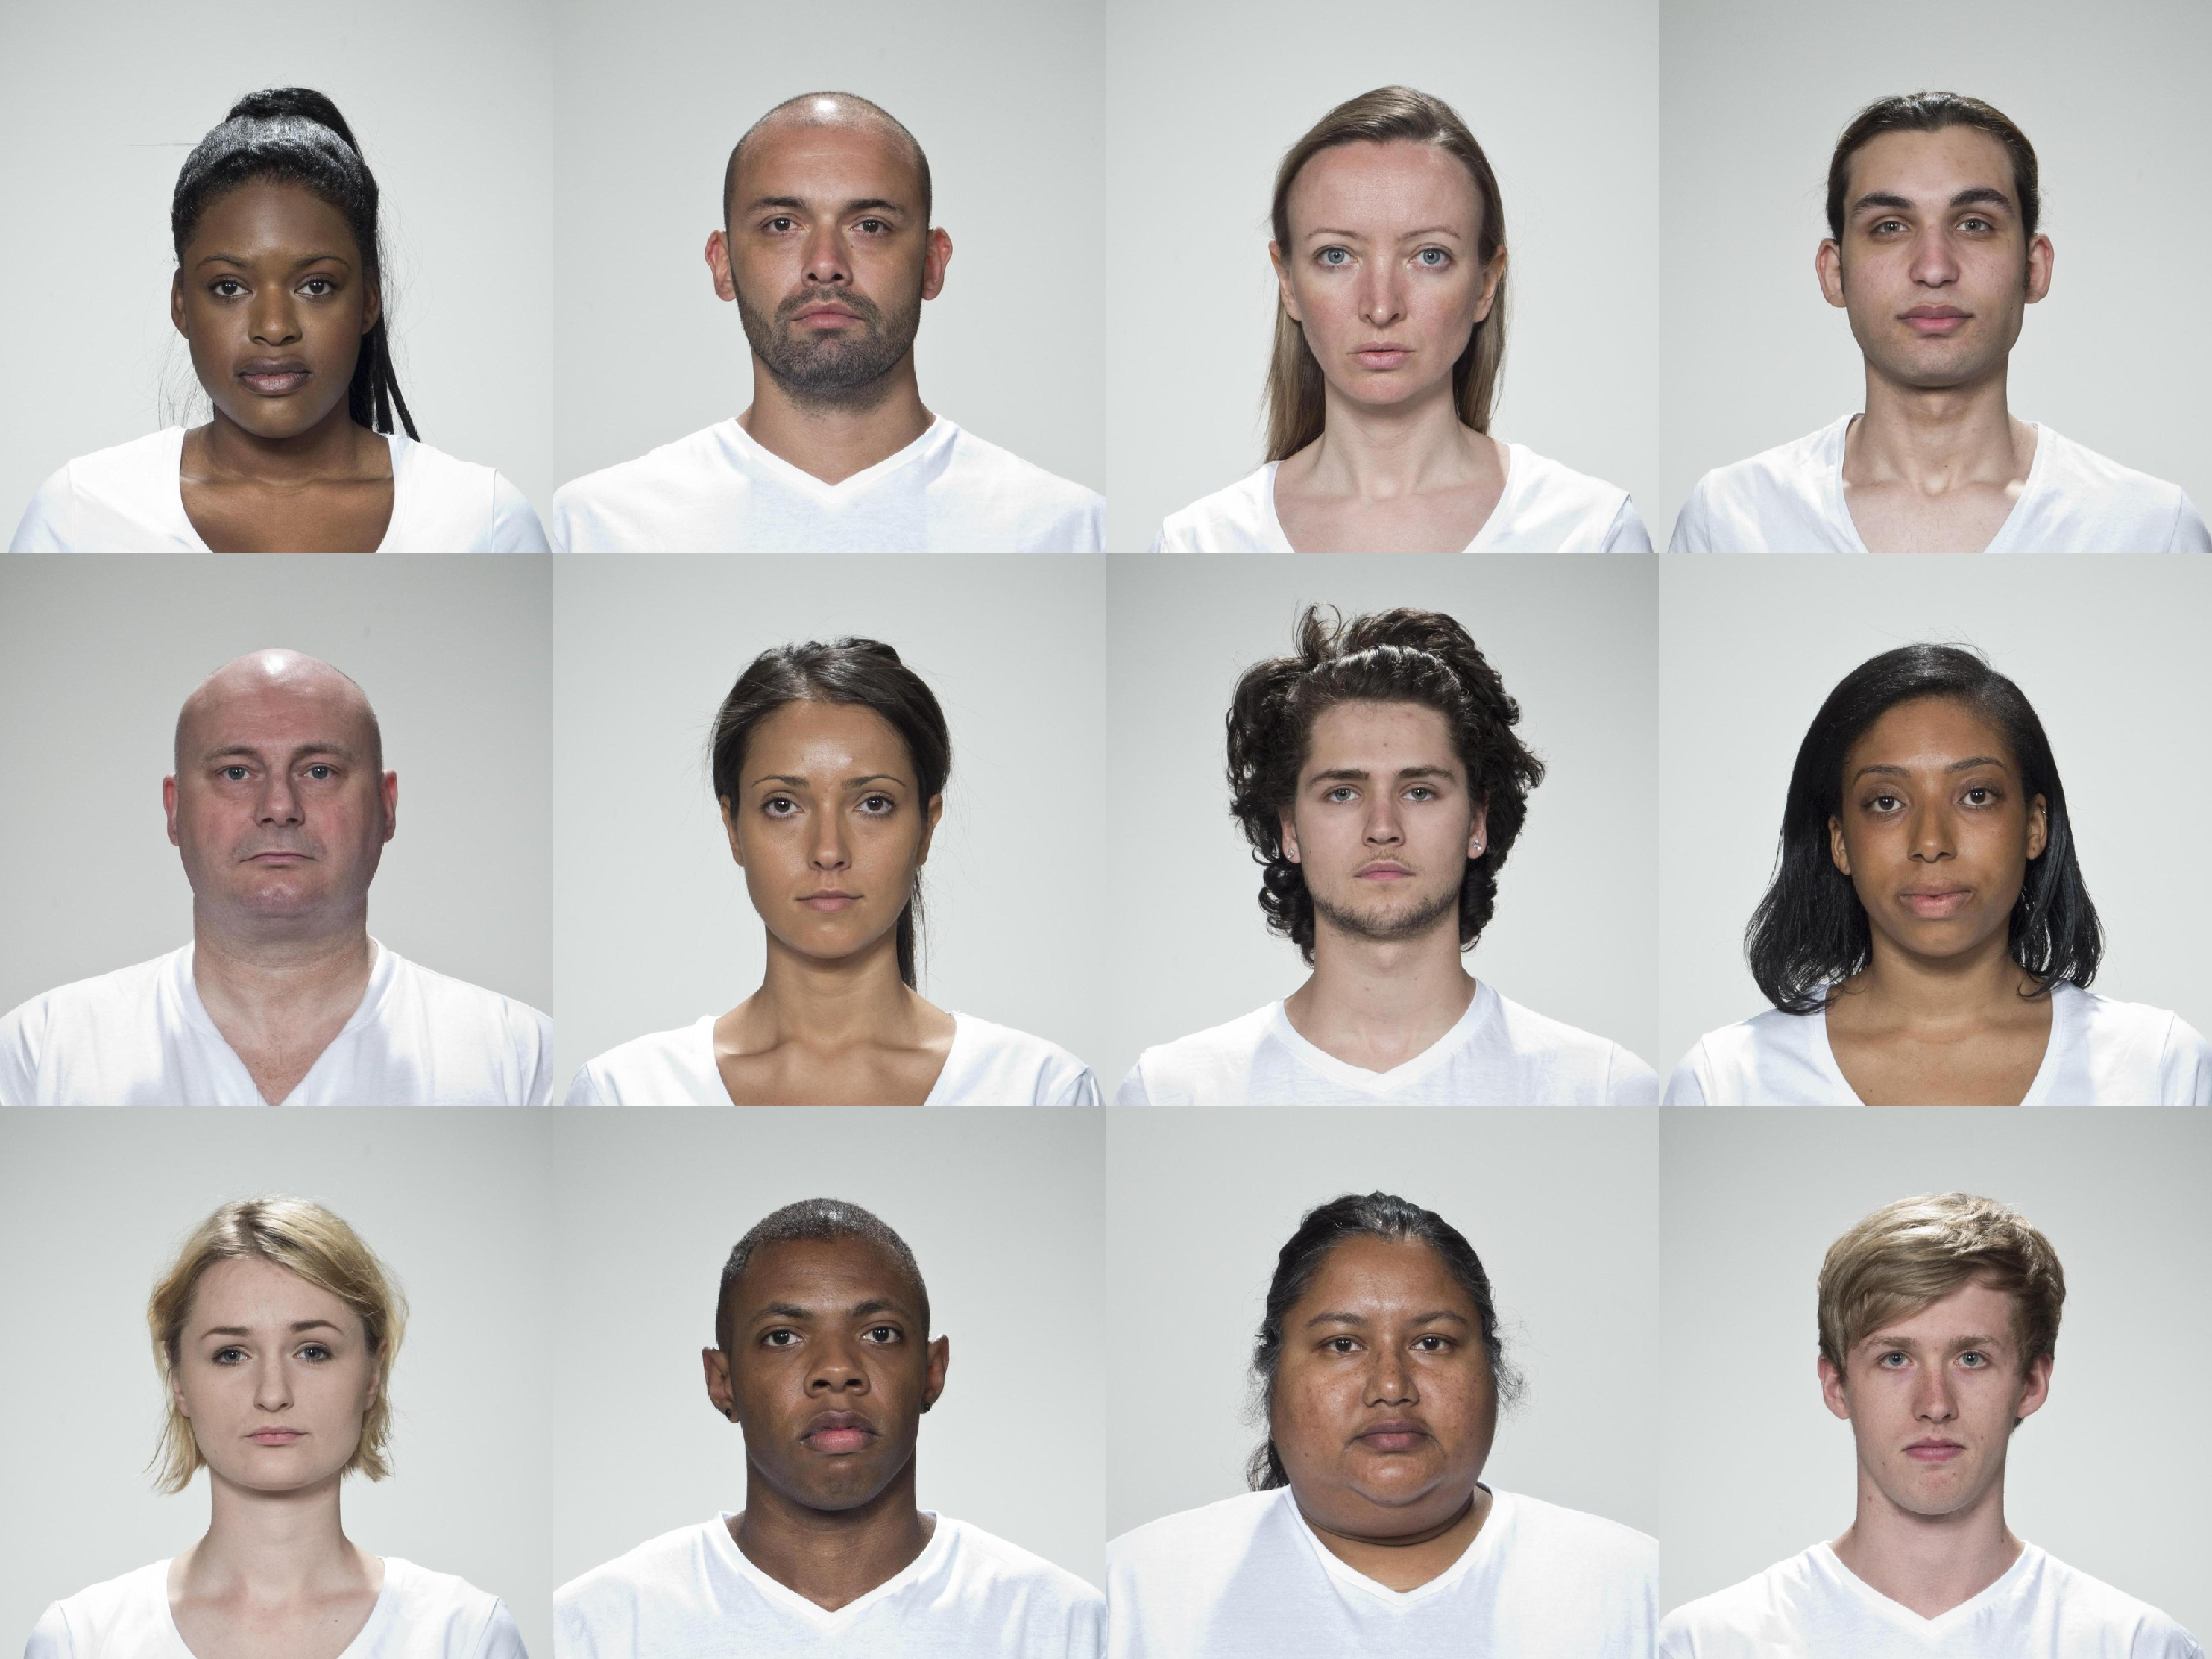
\includegraphics[width=\textwidth]{images/mos_train_set.pdf}\\
        \caption{MOS train set}\label{fig:mos_set_train}
    \end{subfigure}
    \hfill
    \begin{subfigure}[t]{0.19\textwidth}
        \centering
        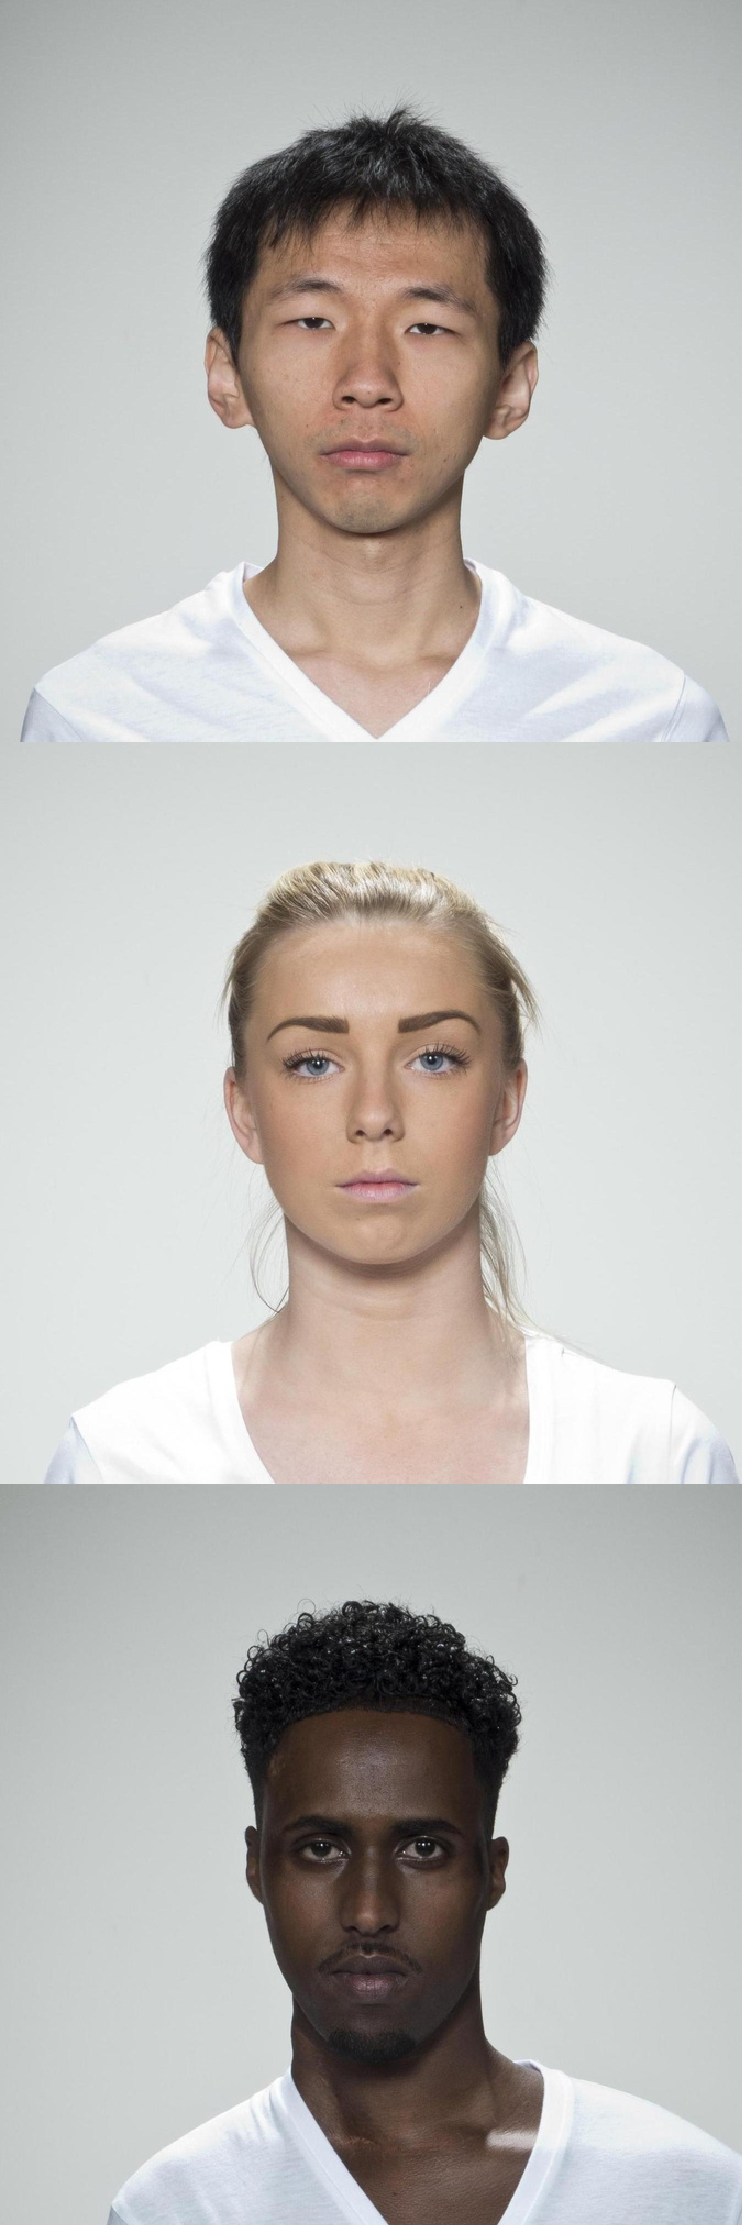
\includegraphics[width=\textwidth]{images/mos_test_set.pdf}\\
        \caption{MOS test set}\label{fig:mos_set_test}
    \end{subfigure}
    \caption{Reference images from the MOS set, comprising the selected subjects from the FRLL dataset.}\label{fig:mos_set}
\end{figure}

The steganographic distortions are visible in Fig.~\ref{fig:steganography}, which shows examples of distorted facial images from each method. The distortions are applied to the original images, and the resulting stego images are used for both subjective evaluation and training of the NR-IQA model.

\begin{figure}[ht]
    \centering
    \begin{subfigure}[t]{0.22\textwidth}
        \centering
        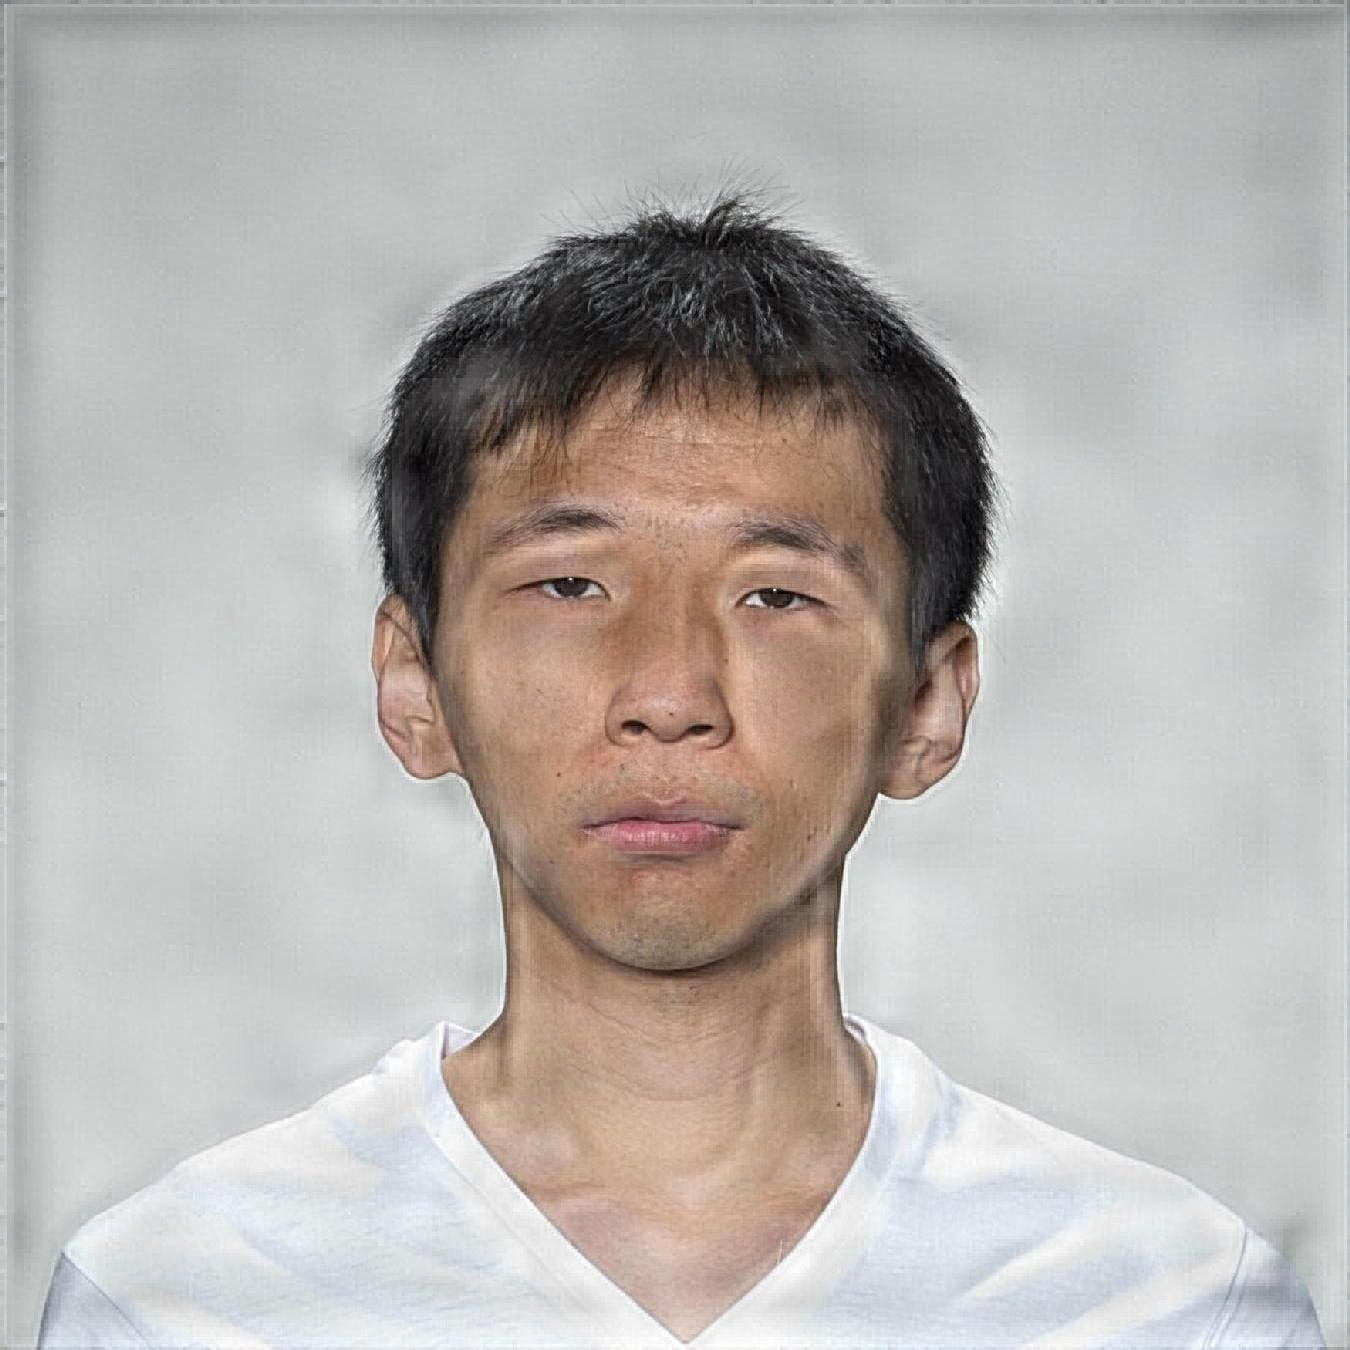
\includegraphics[width=\textwidth]{images/005_StegaStamp_1.4.jpg}\\
        \caption{StegaStamp}\label{fig:steganography_a}
    \end{subfigure}
    \hfill
    \begin{subfigure}[t]{0.22\textwidth}
        \centering
        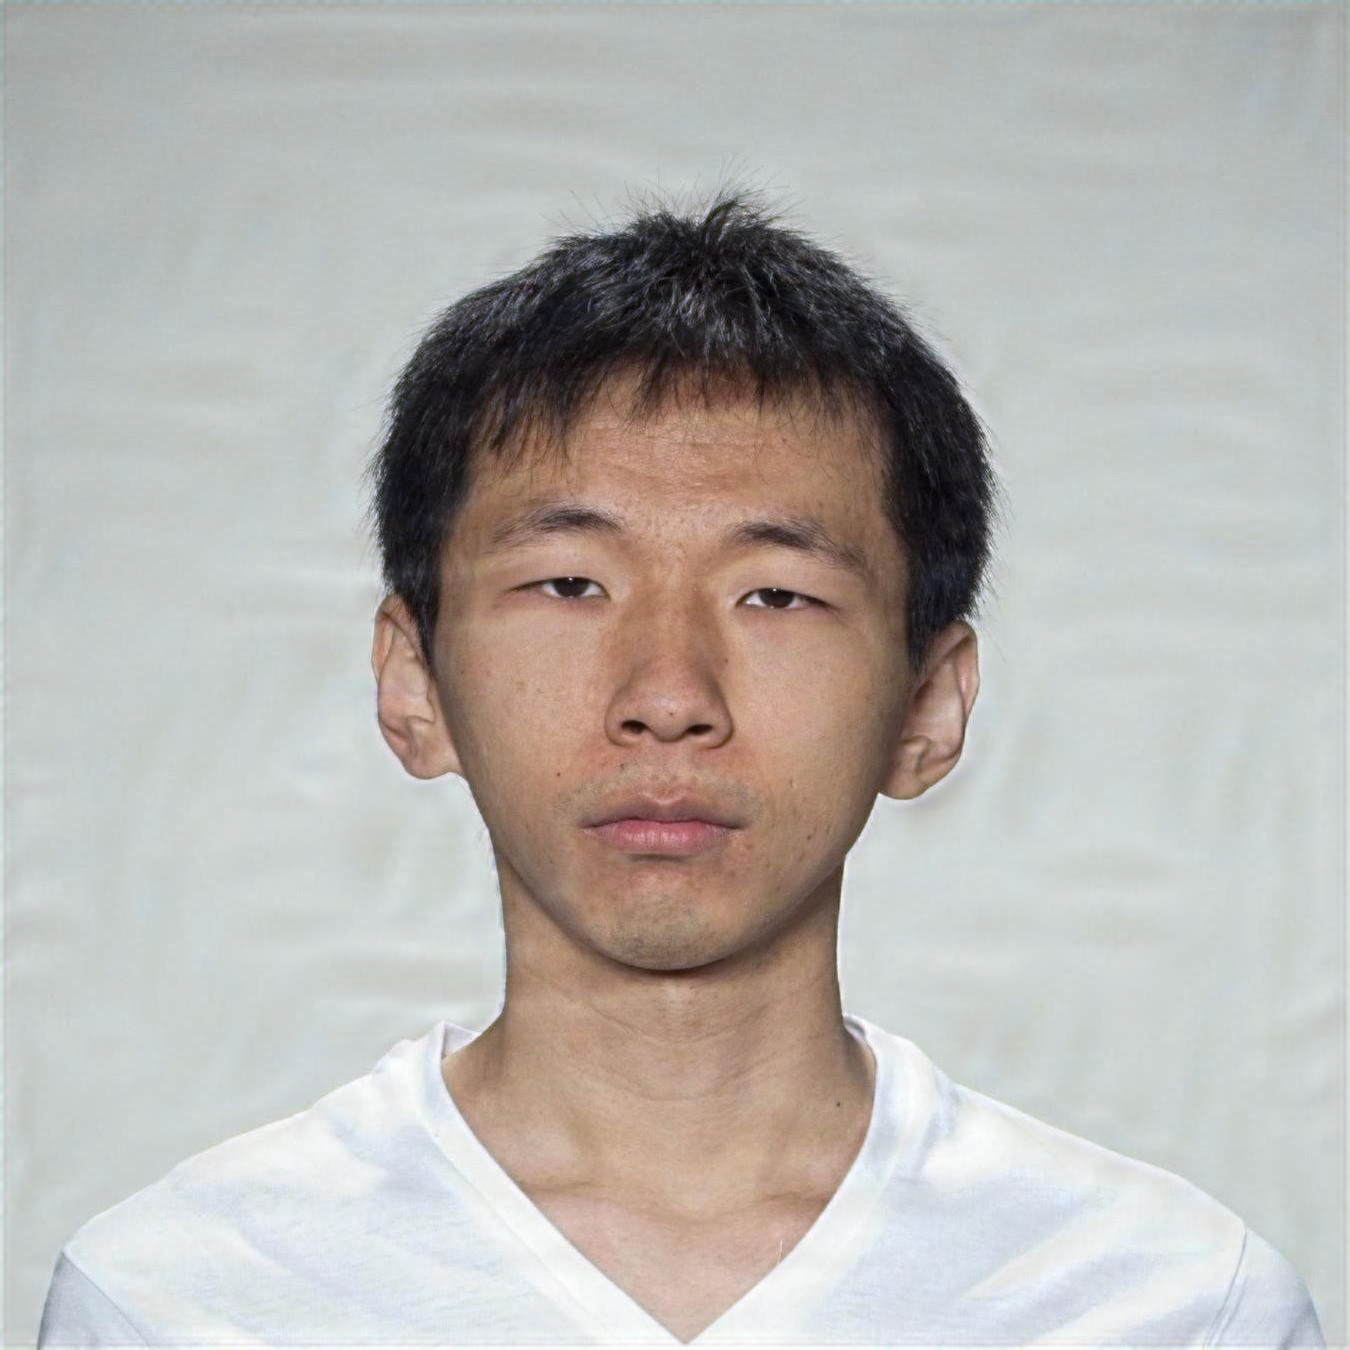
\includegraphics[width=\textwidth]{images/005_CodeFace_1.4.jpg}\\
        \caption{Code\,Face}\label{fig:steganography_b}
    \end{subfigure}
    \hfill
    \begin{subfigure}[t]{0.22\textwidth}
        \centering
        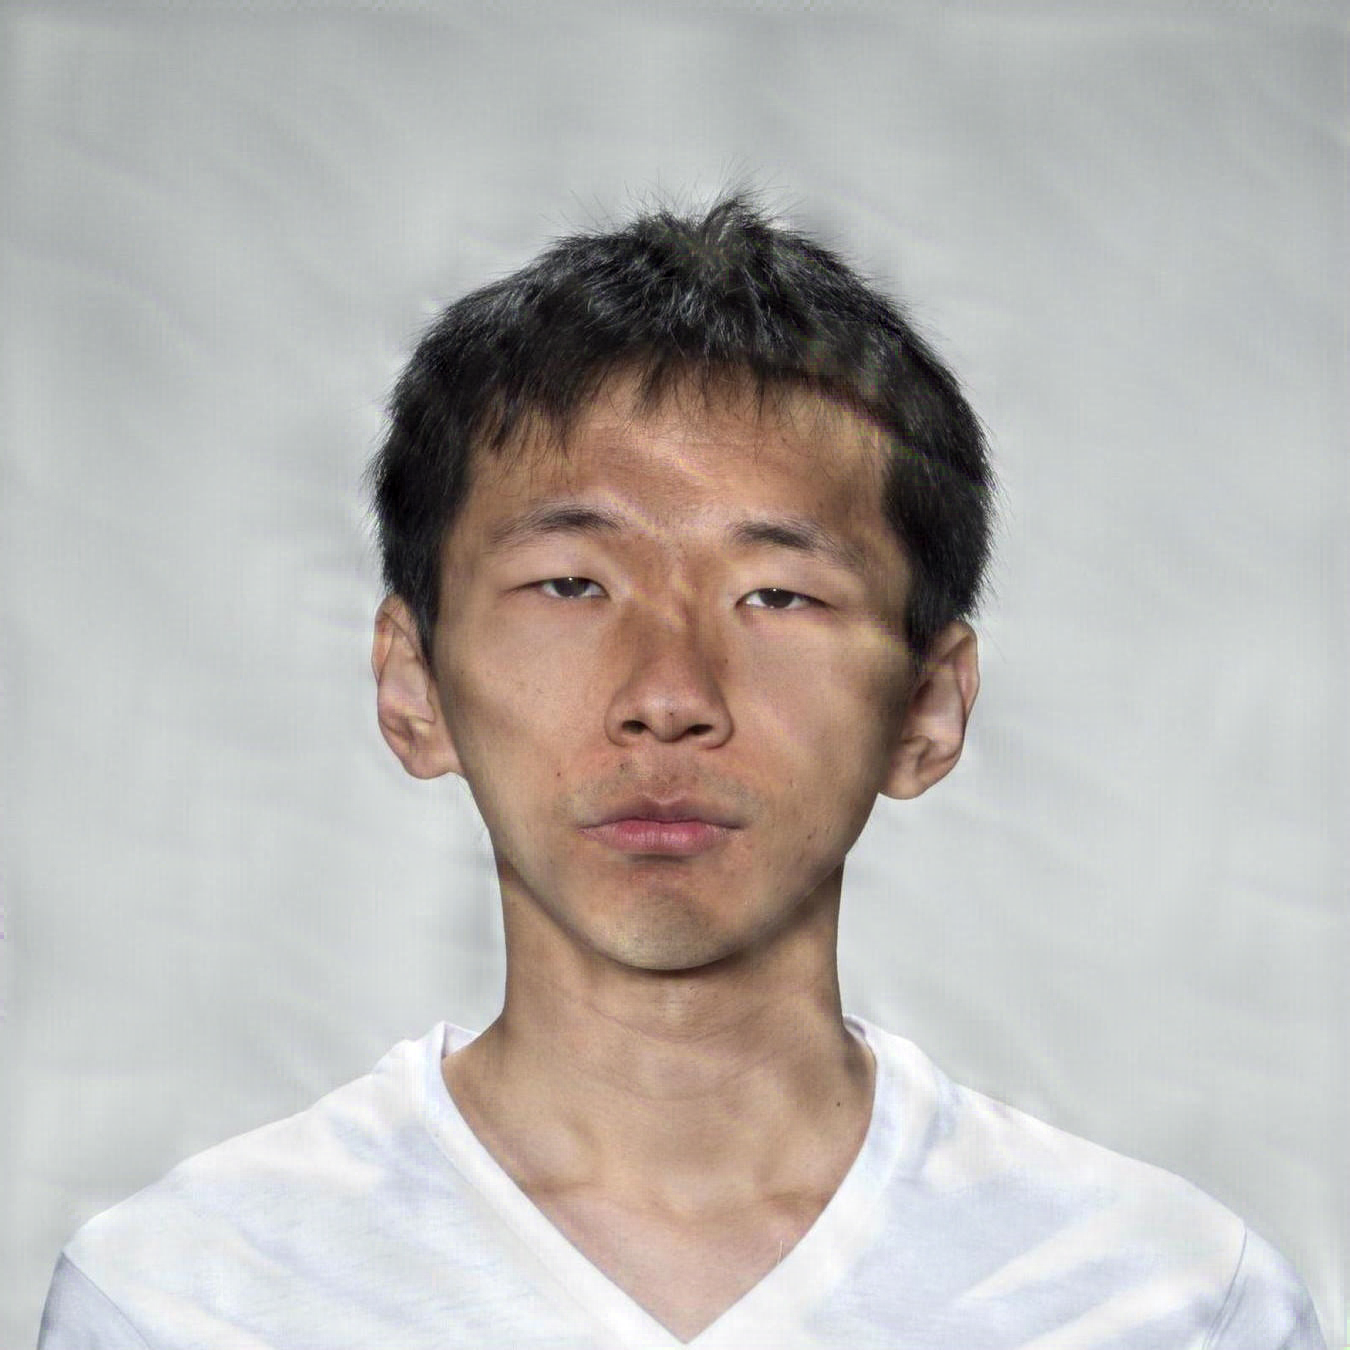
\includegraphics[width=\textwidth]{images/005_RiemStega_1.4.jpg}\\
        \caption{RiemStega}\label{fig:steganography_c}
    \end{subfigure}
    \hfill
    \begin{subfigure}[t]{0.22\textwidth}
        \centering
        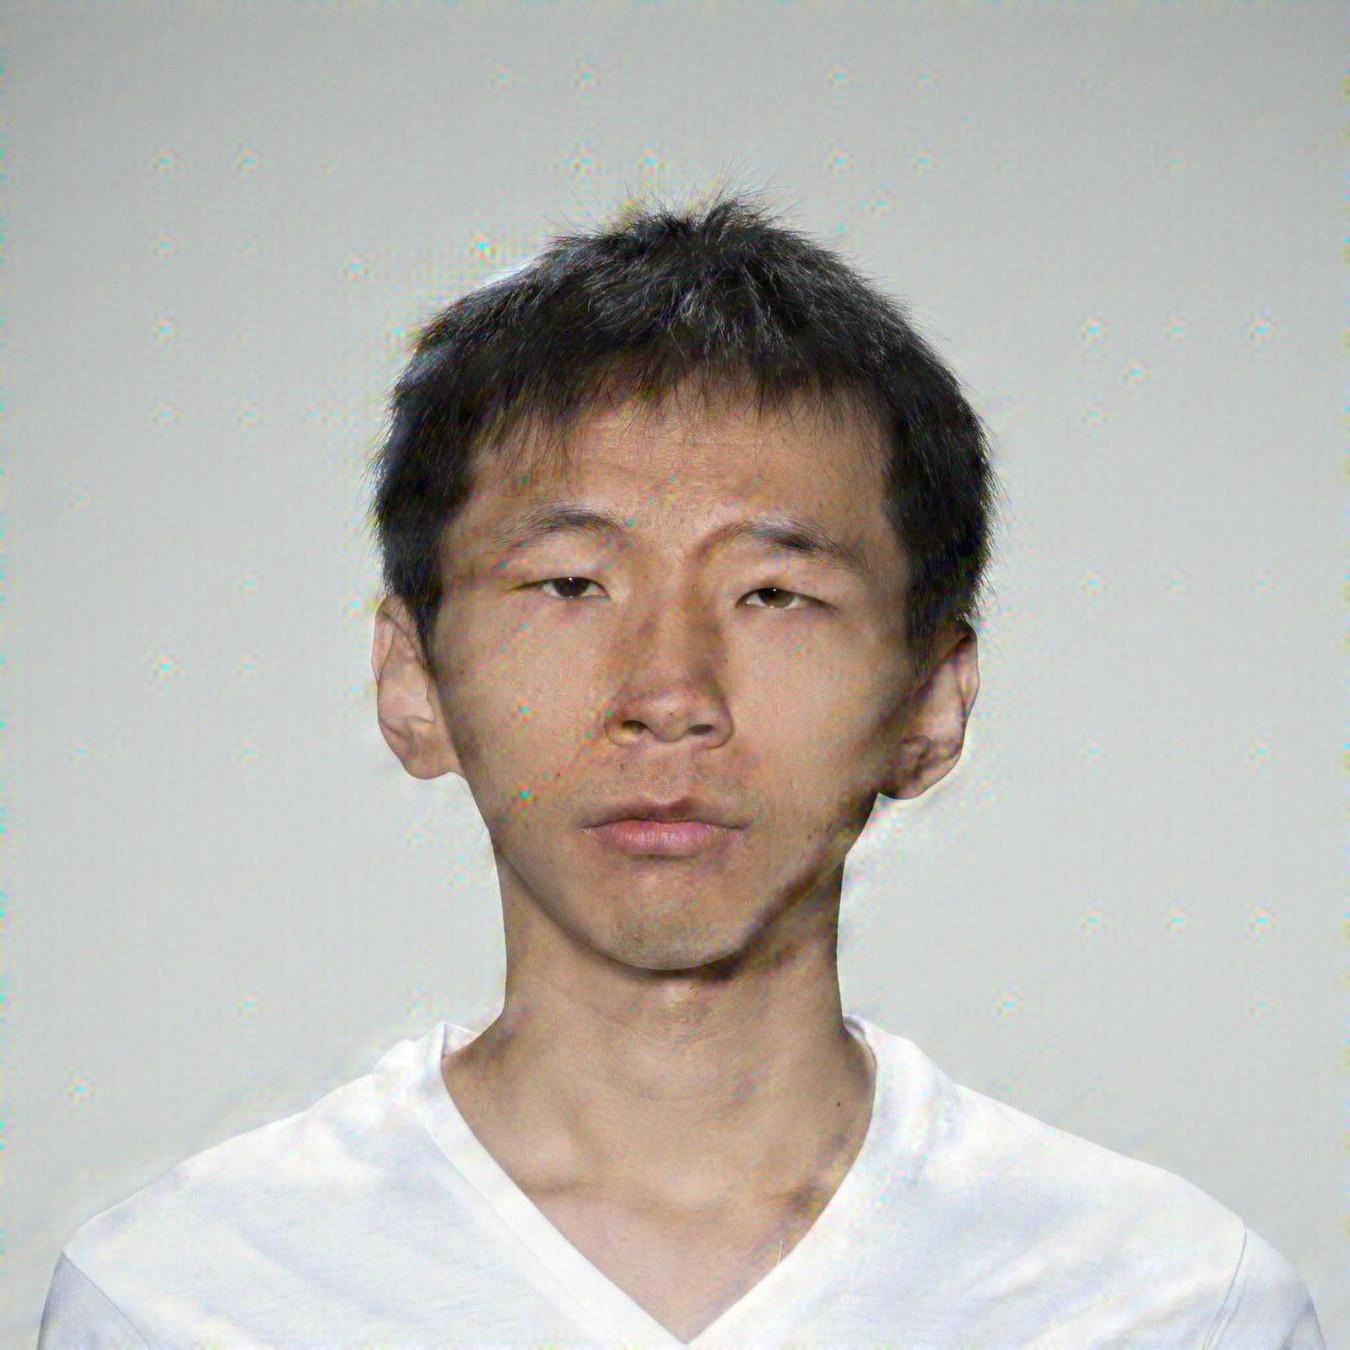
\includegraphics[width=\textwidth]{images/005_StampOne_1.4.jpg}\\
        \caption{StampOne}\label{fig:steganography_d}
    \end{subfigure}
    \caption{Steganographically distorted facial images from each method.}\label{fig:steganography}
\end{figure}

\section{Collection of Subjective Scores}

We followed the ITU-R BT.500--15~\cite{ITU-R-BT500} recommendation and adopted the Single Stimulus (SS) method. The test was implemented using a custom Django web application seen in Fig.~\ref{fig:webapp}. Prior to the test session, participants signed an informed consent form and filled out a registration form providing demographic and environmental information such as age, gender, education, country of origin and ethnicity, and others. Each image was shown individually, with no time limit. Ratings were submitted using a labeled slider, and automatic saving ensured session robustness.

Each image in the MOS set was evaluated approximately 30 times by human observers, resulting in over 14,000 ratings. We had around 200 participants, each session lasted about 22 minutes and included roughly 70 evaluations. Following the session, outlier observers were identified and removed using both Kurtosis-based and correlation-based post-screening methods described in ITU-R BT.500--15~\cite{ITU-R-BT500}, resulting in the exclusion of one participant.

\begin{figure}
    \centering
    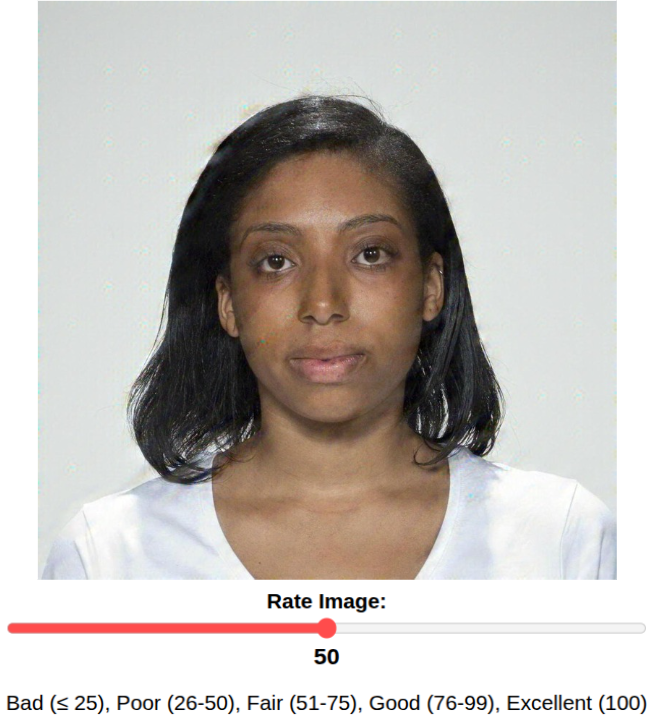
\includegraphics[width=0.32\textwidth]{images/webapp_test.png}
    \caption{Django-based webapp created for the Single Stimulus test.}\label{fig:webapp}
\end{figure}

The database was implemented using the Django web framework, which provides an object-relational mapping (ORM) layer that directly maps Python model classes to database tables. The ORM also enforces data integrity constraints and simplifies querying for statistical analysis. The database backend used was PostgreSQL.

The database schema was designed to ensure structured storage and traceability of all subjective quality evaluation data. Fig.~\ref{fig:db_conceptual} presents the conceptual data model, which defines the main entities and their relationships. The profile entity stores participant metadata, including age, gender, education, ethnicity, country, and device used. The ss\_session entity models individual test sessions and is linked to both the participant profile and the dataset being evaluated. The image entity encodes each image's filename, associated distortion type (distortion\_name), and distortion level (distortion\_level). The test entity stores individual subjective ratings, including the precise timestamp of submission, linked to both the session and the image presented. An auxiliary user\_feedback entity captures optional, anonymous, observer comments and critiques.

The physical implementation of this schema, shown in Fig.~\ref{fig:db_physical}, is realized as a relational database with explicit foreign key constraints to ensure referential integrity. The dataset\_id and profile\_id fields in ss\_session formally enforce the linkage to specific datasets and participants. The test table connects each subjective rating to its session (ss\_session\_id) and image (image\_id), enabling consistent aggregation of ratings into a statistical descriptors such as MOS and confidence intervals per image and per distortion level. The relational model also facilitates efficient querying for downstream statistical analysis and supports reproducibility of the experimental protocol in line with ITU-R BT.500-15 recommendations.

\begin{figure}
    \centering
    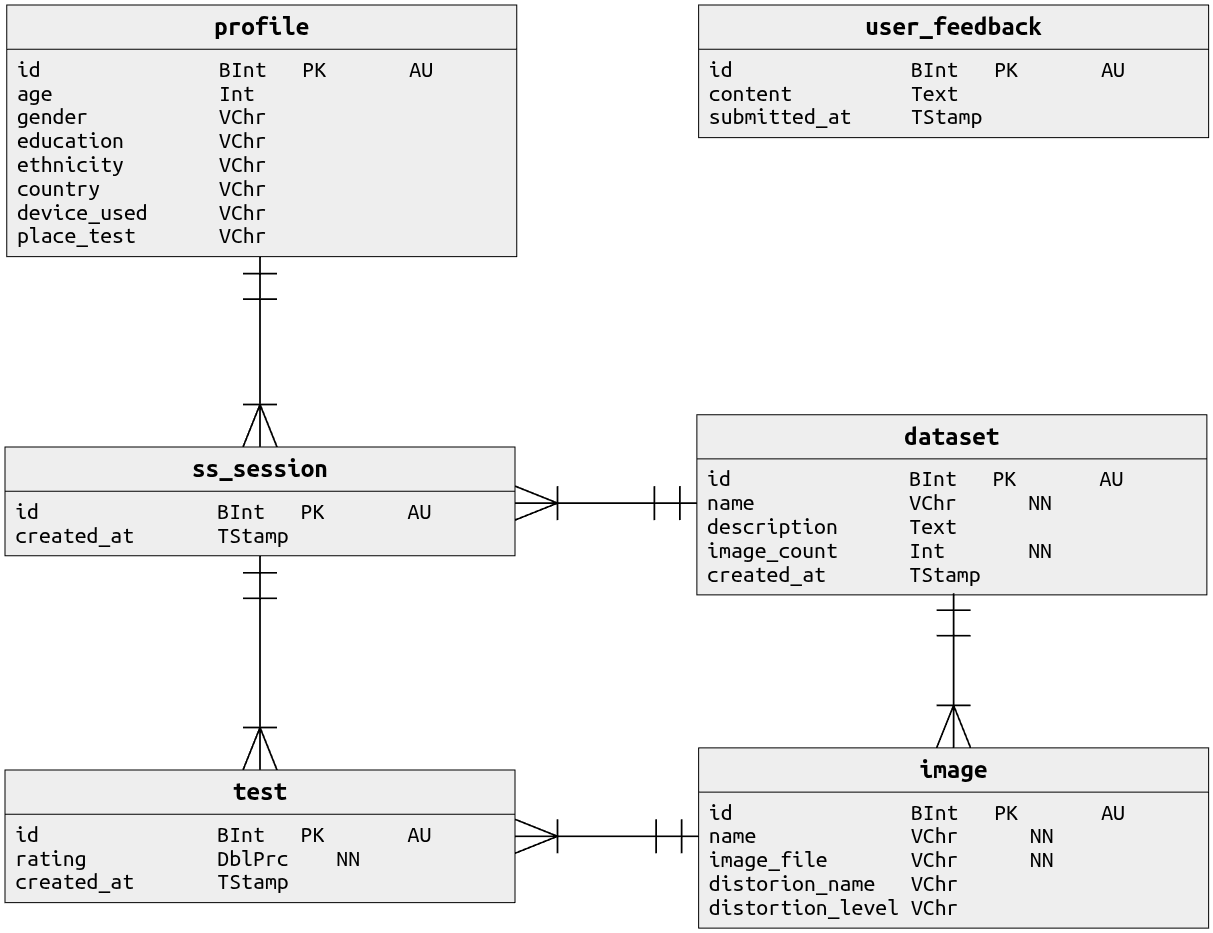
\includegraphics[width=0.8\textwidth]{images/db_conceptual.png}
    \caption{Conceptual database schema.}\label{fig:db_conceptual}
\end{figure}

\begin{figure}
    \centering
    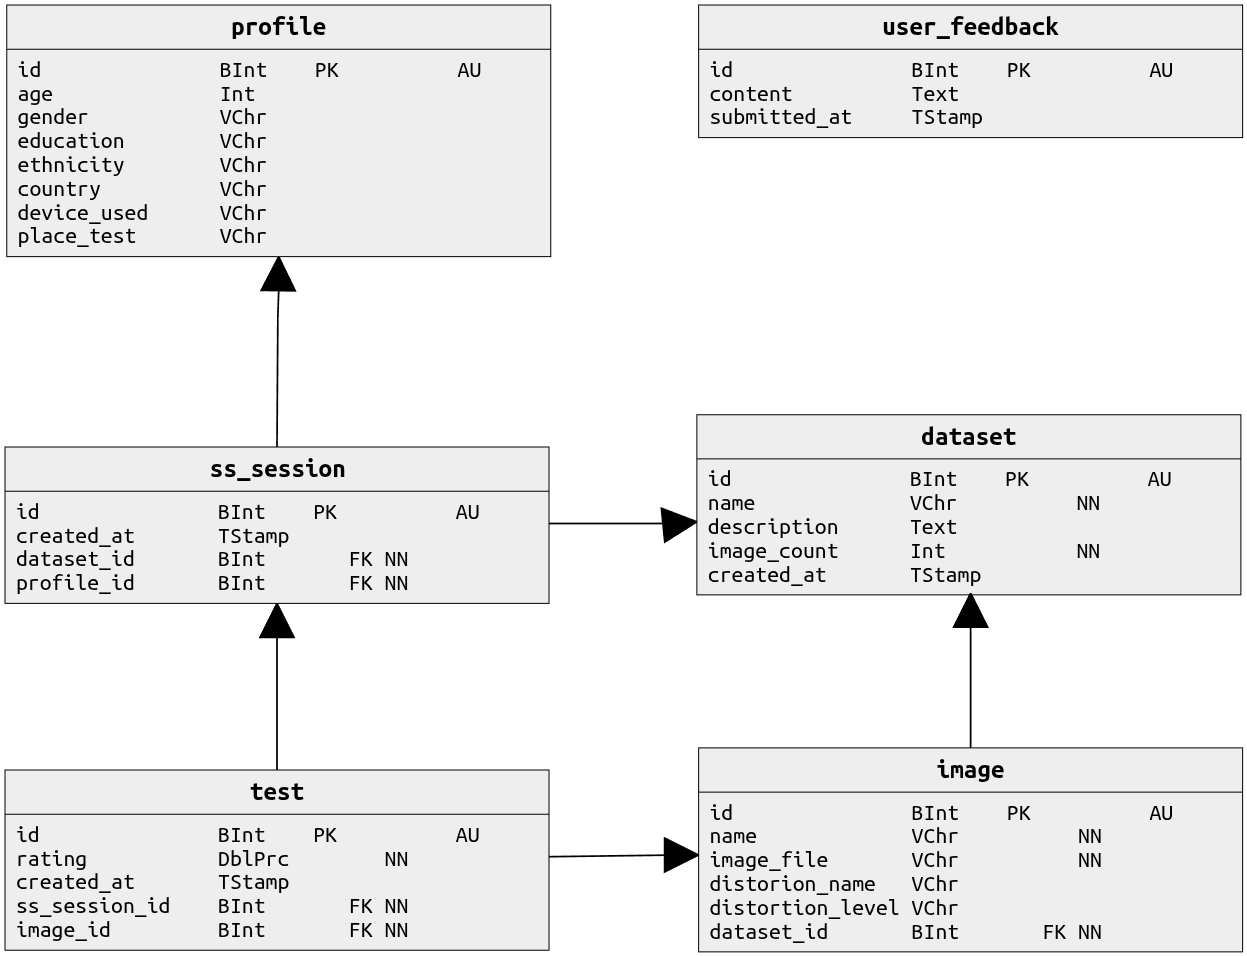
\includegraphics[width=0.8\textwidth]{images/db_physical.png}
    \caption{Physical database schema.}\label{fig:db_physical}
\end{figure}


\section{Debiasing of Subjective Scores}

To correct for demographic bias in the subjective scores, we followed a procedure inspired by prior work on bias correction in perceptual tasks~\cite{clapes2018apparent}, where we applied a residualization method based on linear modeling. An ordinary least squares (OLS) regression was fit to the MOS values, using observer and image attributes, and their pairwise interactions as categorical predictors. The fitted bias components were subtracted from the original scores, and the residuals were mean-centered to preserve the global score distribution. As shown in Table~\ref{tab:anova}, several factors exhibit statistically significant effects on the MOS prior to residualization, notably observer and subject ethnicity. After applying the residualization procedure, these effects disappear, as confirmed by an ANOVA test showing no significant impact from any individual factor. The corrected MOS labels are then used as ground truth in all supervised stages of the pipeline to ensure fairness and reduce the influence of socially conditioned priors.

\begin{table}
    \centering
    \caption{ANOVA~\cite{ross2017one} results for observer and image attributes. Before debiasing, several factors show statistically significant effects on MOS, p-value $< 0.05$.\@ After residualization, all main effects show no significant impact, confirming the effectiveness of the debiasing procedure.}\label{tab:anova}
    \begin{tabular}{lcc}
        \hline % chktex 44
        Factor & p-value & p-value (residualized) \\
        \hline % chktex 44
        Observer gender                             & 0.022                 & 0.9930 \\
        Observer ethnicity                          & $8.44 \times 10^{-4}$ & 1 \\
        Subject gender                              & $1.60 \times 10^{-3}$ & 0.9722 \\
        Subject ethnicity                           & $7.36 \times 10^{-3}$ & 1 \\
        Observer gender $\times$ Subject gender     & 0.6417              & 0.6417 \\
        Observer ethnicity $\times$ Subject ethnicity & 0.0582              & 0.0582 \\
        \hline % chktex 44
    \end{tabular}
\end{table}

\section{Correlation of FR-IQA Metrics with Human Perception}

We compute 40 FR-IQA scores for each distorted image in the dataset and compare them against the corresponding MOS, as seen in Fig.~\ref{fig:mos_vs_iqa}. Several metrics exhibit strong linear trends with MOS, while others are poorly aligned or even negatively correlated. For a detailed description of these metrics, we refer the reader to~\cite{shahrukh2019survey}.



\begin{figure}
    \centering
    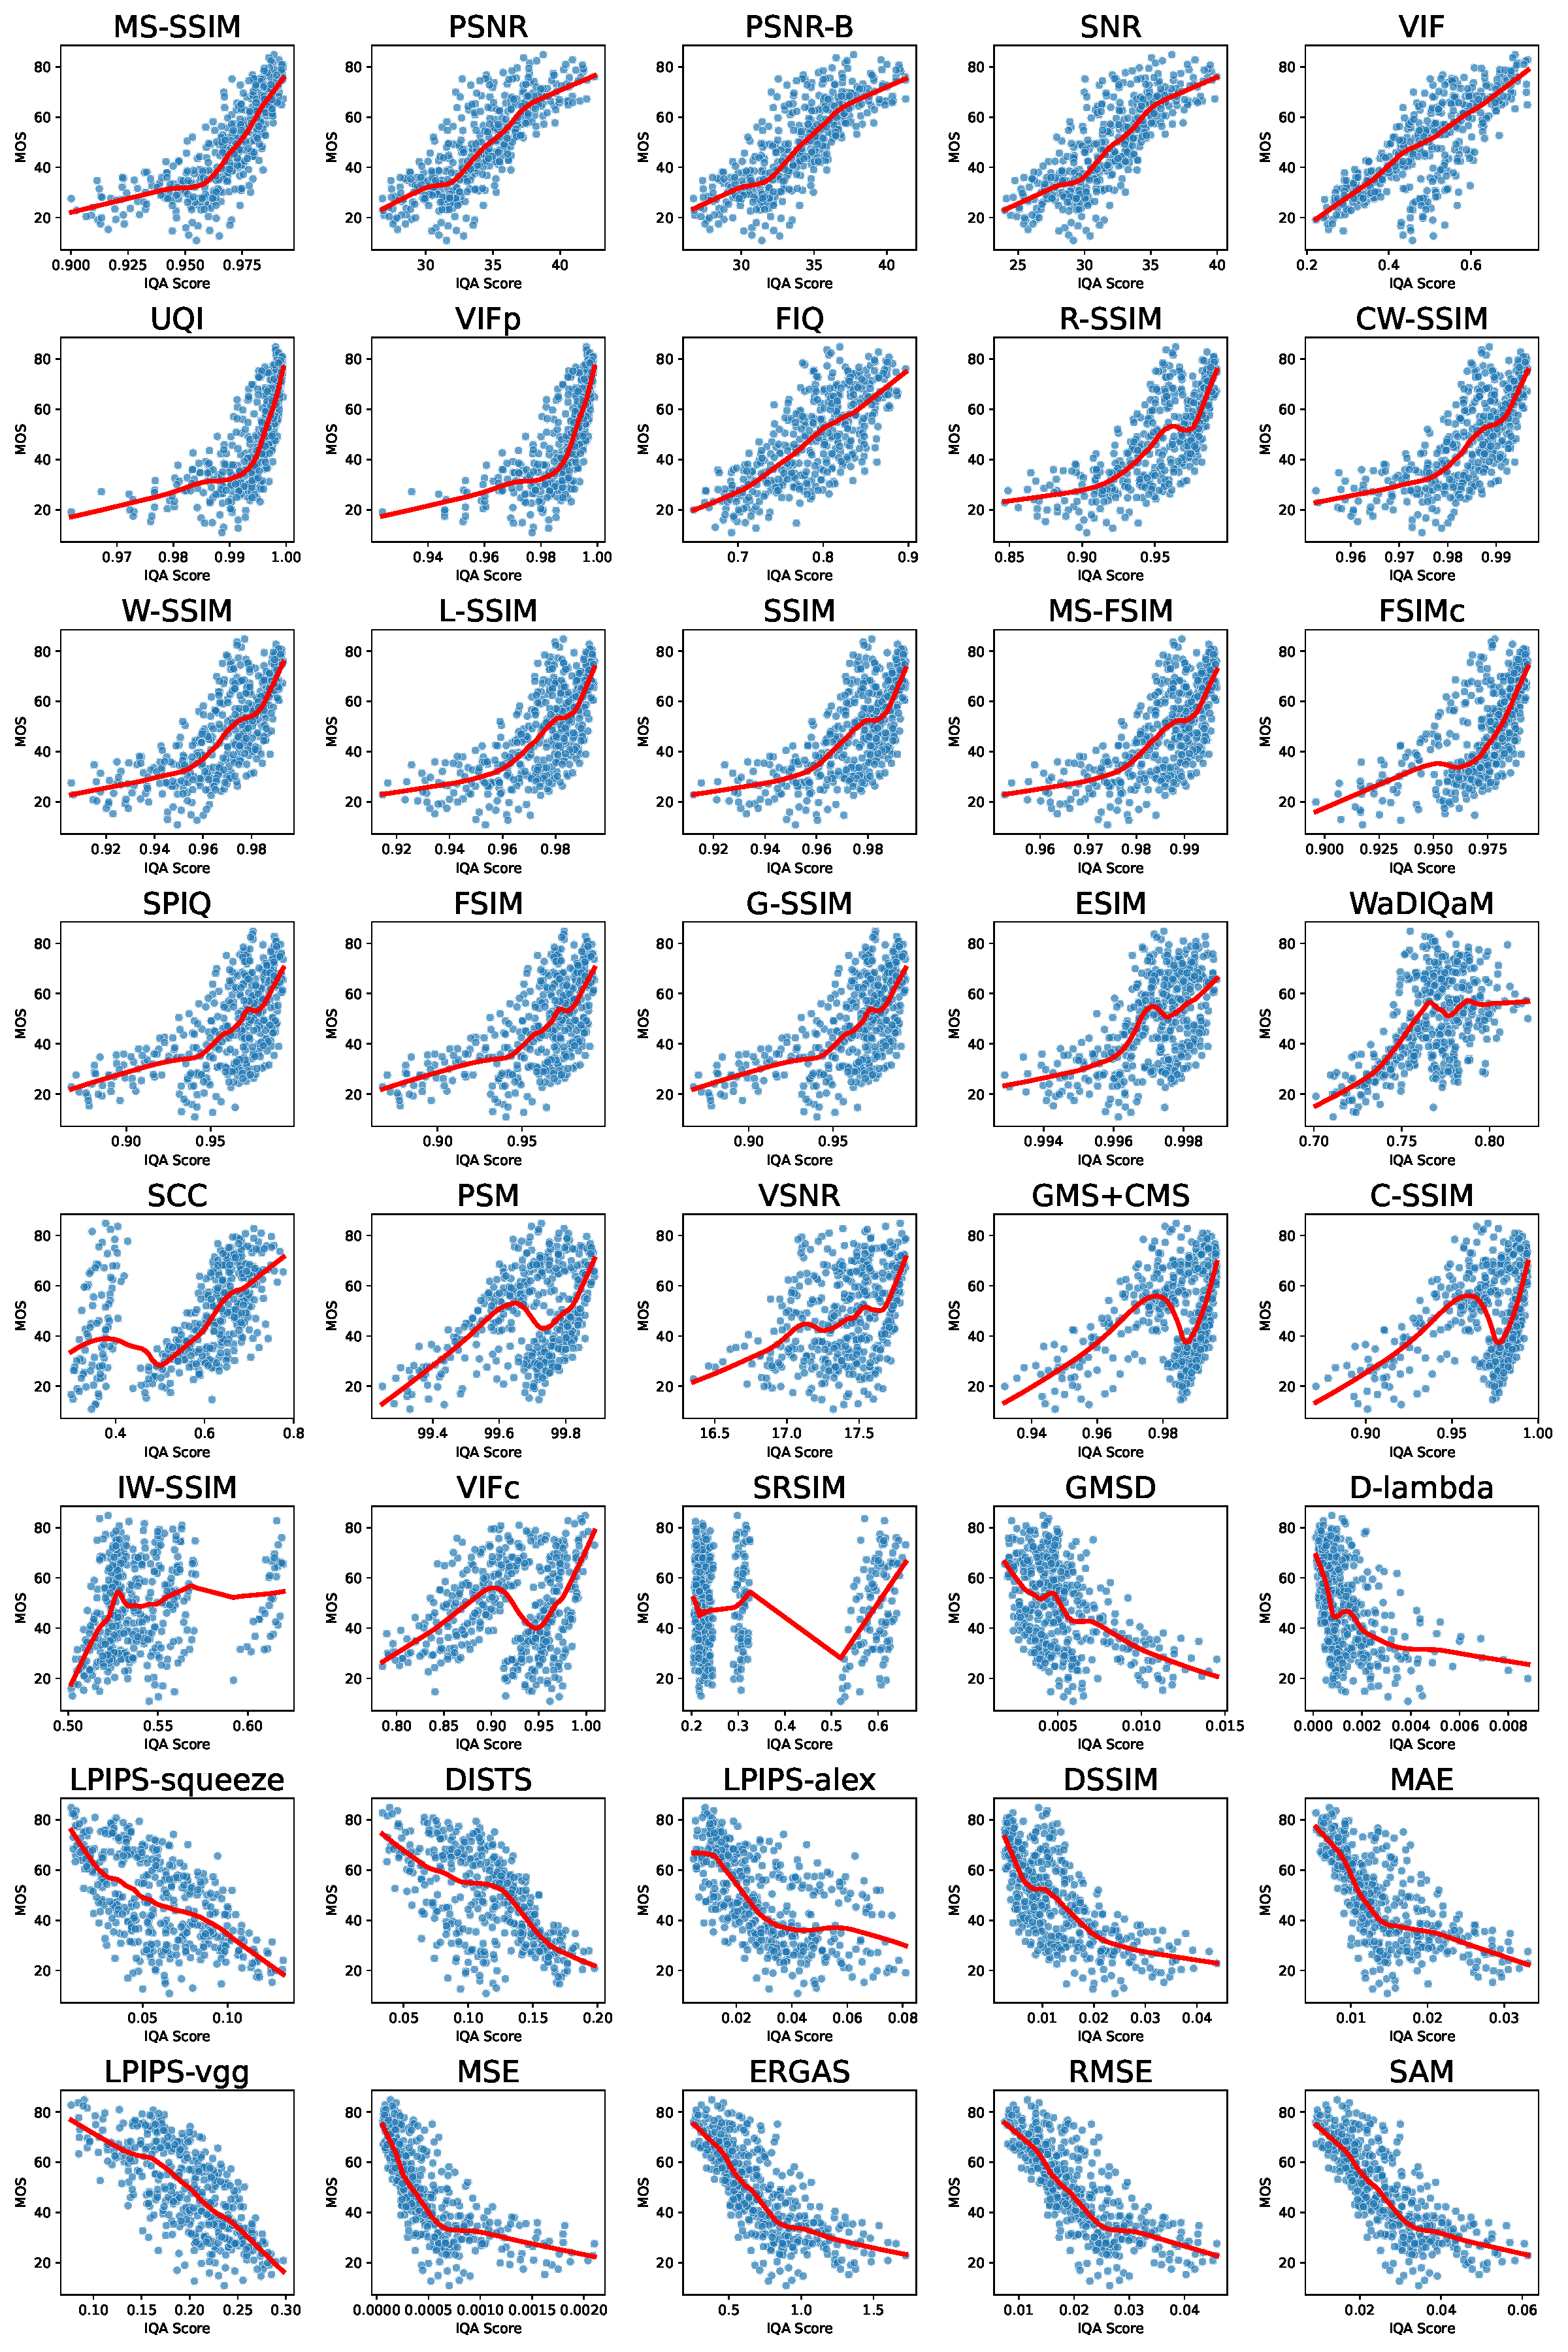
\includegraphics[width=0.90\linewidth]{images/mos_vs_iqa_grid.pdf}
    \caption{Scatter plots illustrating the relationship between MOS and 40 individual full-reference IQA metrics. The red line represents a smoothed local trend curve.}\label{fig:mos_vs_iqa}
\end{figure}

\section{Fusion of FR-IQA Metrics for Pseudo-MOS Estimation}

To identify which metrics align best with human perception, we compute both the Pearson Linear Correlation Coefficient (PLCC) and the Spearman Rank-Order Correlation Coefficient (SRCC)~\cite{plcc-srcc} which respectively quantify the linearity and monotonicity of the relationship between metric scores and MOS.\@ To determine the appropriate number of metrics to retain for fusion, we applied Singular Value Decomposition (SVD) and the Picard criterion~\cite{hansen1998picard}. Metrics are first ranked by the average of their PLCC and SRCC with MOS.\@ After normalizing the feature matrix, SVD revealed that six components capture 95\% of the total variance, as shown in Fig.~\ref{fig:svd_analysis}a, indicating an optimal dimensionality of $k=6$.

To validate this truncation point, we examined the Picard plot in Fig.~\ref{fig:svd_analysis}b, which compares singular values with the target projections. The stable ratio in the tail confirms that six components provide a good balance between expressiveness and stability. This supports a compact, informative subset of FR-IQA metrics.

\begin{figure}[ht]
    \centering
    \begin{minipage}[t]{0.48\textwidth}
        \centering
        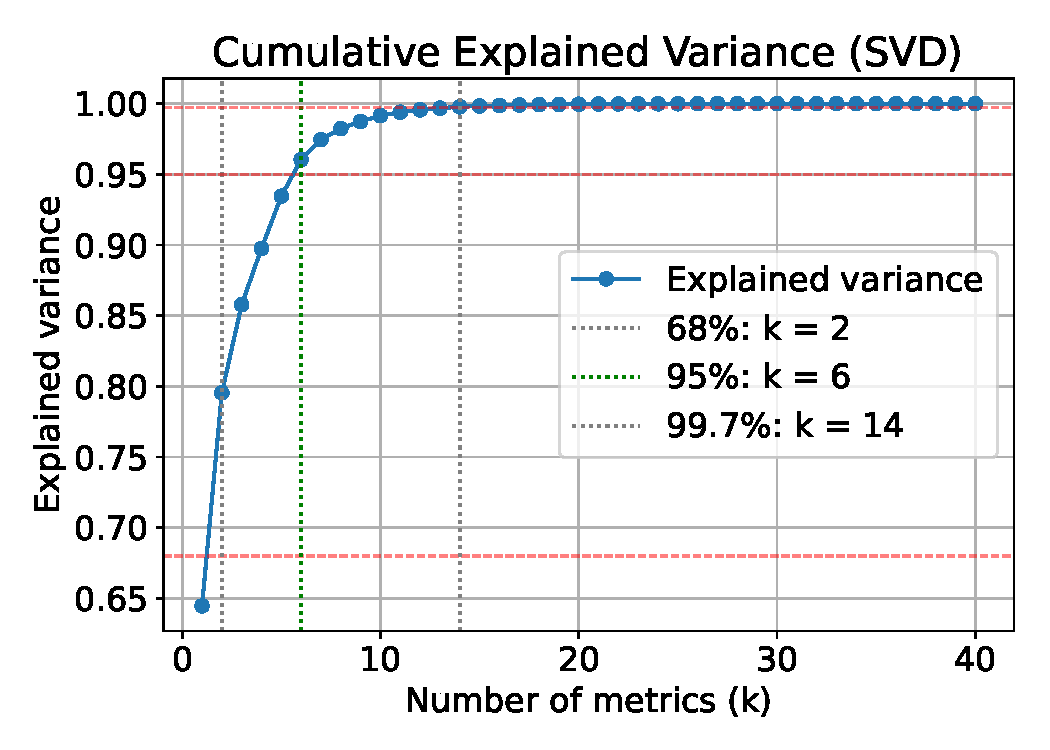
\includegraphics[width=\linewidth]{images/variance.pdf}
        \textbf{(a)} Cumulative variance explained by SVD components.
    \end{minipage}
    \hfill
    \begin{minipage}[t]{0.48\textwidth}
        \centering
        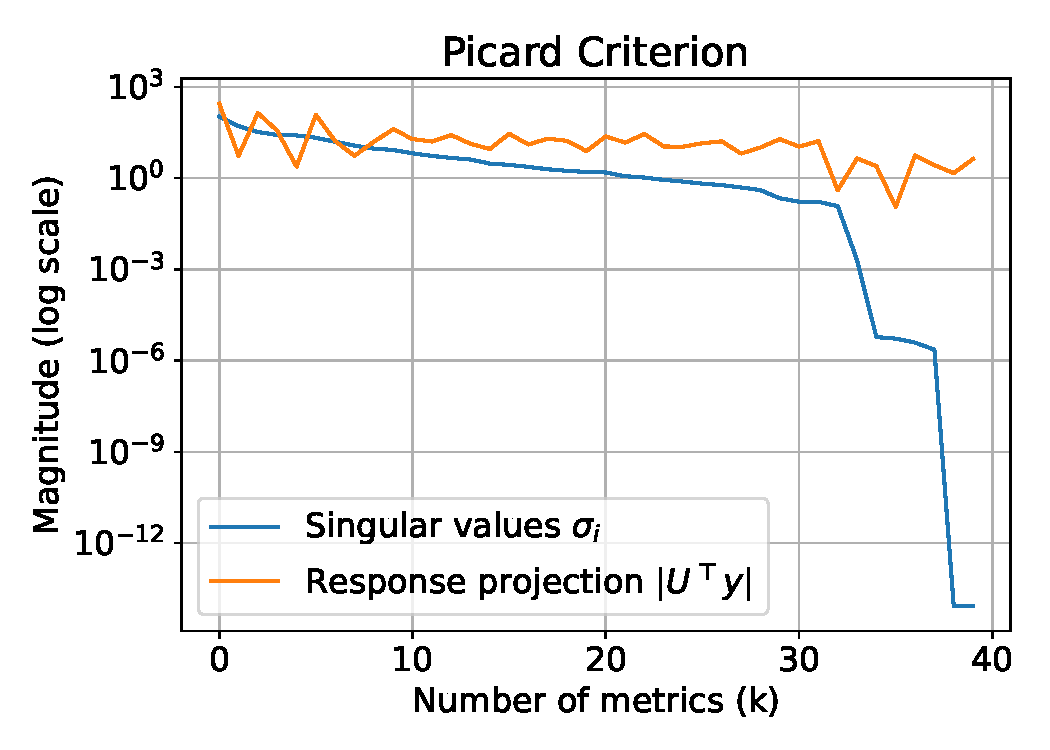
\includegraphics[width=\linewidth]{images/picard.pdf}
        \textbf{(b)} Magnitude of singular values and projected response.
    \end{minipage}
    \caption{SVD-based analysis of the FR metric space. The cumulative explained variance (a) guides the choice of dimensionality, while the Picard criterion (b) illustrates stability near $k=6$.}\label{fig:svd_analysis}
\end{figure}

After selecting the top $k = 6$ FR-IQA metrics, we trained a diverse set of supervised regressors to map these features to subjective MOS scores. The models included both linear and non-linear types:

\begin{itemize}
    \item Linear models: Linear Regression~\cite{linearregression}, Ridge Regression~\cite{ridgeregression}, Bayesian Ridge~\cite{bayesianridge}, ElasticNet~\cite{elasticnet}.
    \item Kernel-based: Support Vector Regression~\cite{svr} (SVR).
    \item Ensembles: Random Forest~\cite{randomforest}, Extra Trees~\cite{ensembles}, Gradient Boosting~\cite{gradboosting}, HistGradientBoosting~\cite{histboost}.
    \item Boosted Trees: XGBoost\cite{xgboost}, LightGBM~\cite{lightgbm}, CatBoost~\cite{catboost}.
\end{itemize}

Each regressor was trained using five-fold cross-validation with an exhaustive grid search over predefined hyperparameter spaces. The best model, CatBoost, optimal configuration was: depth = 8, iterations = 500, learning rate = 0.05, and $L_2$ regularization = 1. This trained regressor is then applied to the unlabeled portion of the dataset (3,132 distorted images), generating pseudo-MOS.\@

\section{Training a No-Reference IQA Model from Pseudo-MOS}

To enable NR quality prediction, we train a deep regression model end-to-end using pseudo-MOS scores as targets. The architecture is based on a ResNet-18 backbone~\cite{resnet} pretrained on ImageNet~\cite{imagenet}, with its final classification layer replaced by a lightweight multi-layer perceptron (MLP) regressor~\cite{bayesianridge}. All layers are fine-tuned during training to learn perceptual quality representations specific to our task. The training set consists of distorted facial images paired with either pseudo-MOS, from the FR fusion, or real MOS labels, when available. The model is optimized using MSE and evaluated on the, disjoint, MOS test set of labeled images. Once trained, the model infers image quality solely from the distorted input, enabling NR assessment aligned with human perception.


\section{Experimental Setup and Evaluation}

To assess the effectiveness of the proposed method, we conduct qualitative and quantitative evaluations of the generated images.

\subsection{Experimental Setup}

We generate a dataset of augmented icons using a diverse set of textures from \texttt{texture\_pack}. The visibility factor $\alpha$ is varied within the predefined range, and random border expansions are applied. The output images are analyzed for their blending quality and degradation realism.

To ensure a fair evaluation, we consider multiple test cases with different texture types, including smooth, rough, and highly creased surfaces. Additionally, we vary the positioning of the icons to test the robustness of the algorithm against different spatial placements.

\subsection{Qualitative Evaluation}

Sample images generated using the proposed algorithm are visually examined to assess their consistency with real-world degradation effects. As shown in Figure~, the blended icons exhibit natural variations in contrast, smudging, and background integration. The images are compared with real-world printed and degraded icons to validate their visual authenticity.

Furthermore, we analyze how different textures impact the final blended output. Icons placed on highly wrinkled textures show more severe degradation, whereas smoother textures yield more subtle blending effects. These qualitative insights help refine the augmentation process.

\subsection{Quantitative Evaluation}

To quantify the effectiveness of the blending, we compute similarity metrics such as the Structural Similarity Index (SSIM) and Peak Signal-to-Noise Ratio (PSNR) between the augmented icons and real-world degraded icons. Higher SSIM values indicate a closer resemblance to naturally degraded images, while PSNR provides an objective measure of signal distortion.

Additionally, we perform a perceptual evaluation by conducting a user study where participants rate the realism of the generated images on a Likert scale. The user study includes a diverse group of individuals who assess whether the augmented images convincingly mimic real-world degradation. Statistical analysis of the responses provides insights into the subjective quality of the augmentation technique.

\subsection{Results and Discussion}

The evaluation results demonstrate that the proposed method produces highly realistic degraded icons with minimal artifacts. The combination of texture-based blending and height-map-driven degradation ensures that the output images closely resemble real-world printed icons exposed to wear and environmental effects.

Table~ presents a summary of the SSIM and PSNR values for different texture categories. The results indicate that textures with higher roughness lead to lower SSIM scores, which aligns with the expectation that increased degradation reduces structural similarity. However, user study results suggest that these variations contribute positively to the perceived authenticity of the degradation effects.

The findings highlight the strengths of the proposed method in generating realistic augmentations while also identifying areas for further improvement, such as fine-tuning degradation intensity based on specific use cases.


\end{document}
